% *******************************************************************************
% * Copyright (c) 2007 by Elexis
% * All rights reserved. This document and the accompanying materials
% * are made available under the terms of the Eclipse Public License v1.0
% * which accompanies this distribution, and is available at
% * http://www.eclipse.org/legal/epl-v10.html
% *
% * Contributors:
% *    G. Weirich
% *
% *  $Id: elexis-fire.tex 5211 2009-03-16 14:54:56Z rgw_ch $
% *******************************************************************************
% !Mode:: "TeX:UTF-8" (encoding info for WinEdt)

\documentclass[a4paper]{scrartcl}
\usepackage{german}
\usepackage[utf8]{inputenc}
\usepackage{makeidx}
\makeindex

\usepackage[pdftex]{graphicx}
\DeclareGraphicsExtensions{.pdf,.jpg,.png}

\usepackage{floatflt}
\usepackage{wrapfig}
\usepackage[]{hyperref}
\usepackage{color}
\begin{document}
\title{elexis-fire}
\author{Gerry Weirich}
\maketitle

\section{Einführung}
Elexis-fire ist ein Fragment\footnote{Ein 'Fragment' ist in der Eclipse-Terminologie ein 'Plugin-Teilstück'. Es ist also nicht selbständig ablauffähig, sondern nur zusammen mit seinem Stamm-Plugin. Ansonsten ist ein Fragment in jeder Hinsicht einem Plugin gleichzusetzen und wird auch genauso wie ein Plugin in den Ordner 'plugins' installiert.}, welches sich ans Plugin elexis-icpc anhängt. Es implementiert den vom Projekt Fire (http://www.icpc.ch/index.php?id=23) geforderten Export von bestimmten, im Rahmen der Konsultation erhobenen Daten in ein standardisiertes XML-File.

\medskip

Dieses Plugin benötigt Elexis 1.4.1 oder 2.0, sowie die Plugins elexis-befunde und elexis-arzttarife-schweiz (diese Plugins sind in der normalen Standarddistribution enthalten).

\section{Konfiguration}
Bedingt durch die Flexibilität, in der in Elexis Befunde erfasst werden können, kann das Export-Fragment nicht 'wissen', wo Sie beispielsweise den Blutdruck zu notieren pflegen. Sie müssen es ihm also sagen. Dies geschieht in der Einstellungsseite \textsc{Datei-Einstellungen-Datenaustausch-SGAM FIRE (ICPC)} (S. Abb. \ref{fire:fig1}).
\begin{figure}
  % Requires \usepackage{graphicx}
  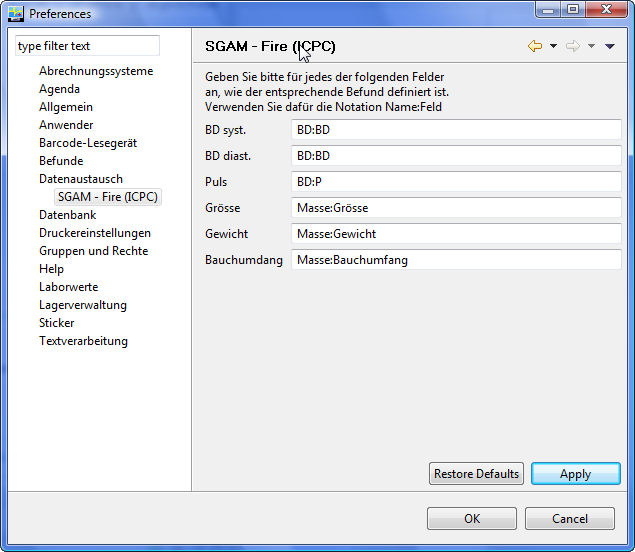
\includegraphics{fire1}\\
  \caption{Fire-Einstellungen}\label{fire:fig1}
\end{figure}

\begin{figure}
  % Requires \usepackage{graphicx}
  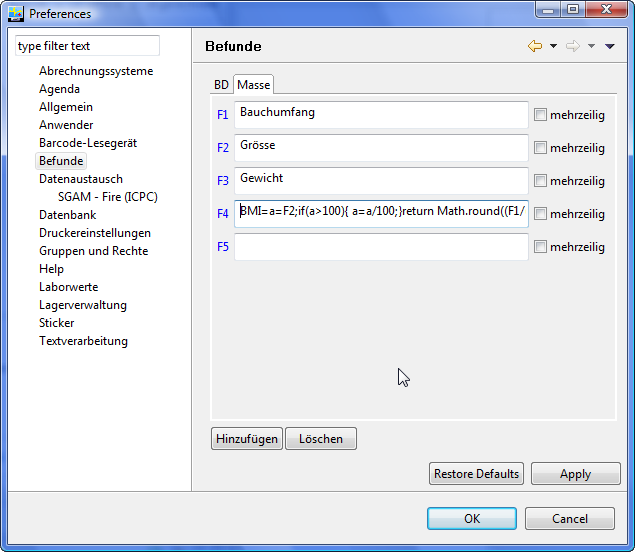
\includegraphics{fire2}\\
  \caption{Befunde-Beispiel}\label{fire:fig2}
\end{figure}

Wie Sie sehen, werden die entsprechenden Befunde mit Termen der Art Karteireiter:Element  deklariert. In Abb \ref{fire:fig2} sehen Sie die zu diesem Beispiel gehörenden Befunde-Voreinstellungen: Es gibt die Karteireiter BD und Masse, bei ersterem die Elemente BD und Puls, bei letzterem die Elemente Grösse usw. Mit der Anweisung Masse:Grösse weisen Sie also in diesem Beispiel den Fire-Exporter an, an dieser Stelle nach dem Eintrag für die Grösse zu suchen. Mehr allgemeine Informationen zur Definition von Befunde-Karteireitern finden Sie im Elexis-Handbuch und auf der Elexis-Website (http://www.elexis.ch/jp/content/view/37/76/).

\medskip

Für den Blutdruck gibt es noch eine Besonderheit zu betrachten: Manche Ärzte erfassen gerne systolischen und diastolischen Blutdruck getrennt als eigene Elemente, während andere den Blutdruck lieber in der Art 120/80 erfassen. Der Fire-Exporter kommt natürlich mit beiden Vorlieben zurecht: Wenn Sie für \textit{BD syst} und \textit{BD diast} dieselbe Deklaration eingeben, dann sucht der Exporter in diesem Feld nach Blutdruckeinträgen der Form syst/diast. Wenn Sie verschiedene Deklarationen angeben, sucht er an diesen Stellen.

\section{Anwendung}
Die Verwendung ist trivial: Wenn das Fragment korrekt installiert worden ist, erscheint ein neuer Button in der Elexis-Toolbar (S. Abb. \ref{fire:fig3}).
\begin{figure}
  % Requires \usepackage{graphicx}
  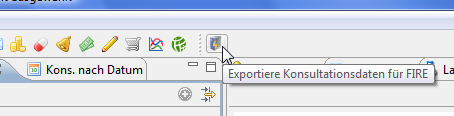
\includegraphics{fire3}\\
  \caption{Fire-Export Button}\label{fire:fig3}
\end{figure}

Nach Klick auf diesen Button öffnet sich eine Dialogbox, in der Sie einen Dateinamen zum Speichern auswählen können. Danach werden alle Konsultationen seit dem 1.1.2009, die bisher noch nicht exportiert wurden, in diese XML-Datei exportiert. Der Transfer der Datei zum Fire-Server ist nicht mehr Gegenstand dieses Plugins; erkundigen Sie sich bitte bei der Projektleitung, auf welchem Weg Sie das File hochladen können.

\bigskip

Anmerkungen:
\begin{itemize}
\item Es werden stets alle Konsultationen seit dem letzten Exportvorgang efasst. Beim ersten Export werden die Konsultationen seit dem 1.1.2009 erfasst.
\item Vitalparameter, Laborwerte, Medikamente etc. werden soweit erfasst, wie sie angegeben sind. Also z.B. ein Blutdruckwert vom 10.3.2009 wird dann exportiert, wenn eine Konsultation vom 10.3.2009 exportiert wird.
\item Zum Export der ICPC-Diagnosen ist es notwendig, dass ICPC-konforme Encounters erstellt werden (Vgl. elexis-icpc-Dokumentation http://www.rgw.ch/elexis/dox/elexis-icpc.pdf). Allerdings erfasst die aktuelle FIRE-Version nur das Segment 'Diagnose' der encounters.
\item Alle exportierten Konsultationen erhalten auch einen (unsichtbaren) Sticker 'Fire', der allenfalls bei späteren Statistiken ausgewertet werden kann. Anhand dieses Stickers wird auch erkannt, wenn eine Konsultation schon einmal exportiert worden ist.
\end{itemize}

\end{document} 